\documentclass[serif,14pt]{beamer}
\usepackage{amsmath, amsfonts, epsfig, xspace}
\usepackage{algorithm,algorithmic}
\usepackage{pstricks,pst-node}
\usepackage{multimedia}
\usepackage{graphicx}
\usepackage[normal,tight,center]{subfigure}
\setlength{\subfigcapskip}{-.5em}
\usepackage{beamerthemesplit}
\usepackage{multirow}
\usepackage[absolute,overlay]{textpos}
  \setlength{\TPHorizModule}{1mm}
  \setlength{\TPVertModule}{1mm}
\usetheme{lankton-keynote}


\author[Group 4]{Stefan Selzer \quad Salil Bhat\\Ioannis Papadopoulos \quad Chang Sun}

\title[Mid-Level Discriminative Patches\hspace{2em}\insertframenumber/\inserttotalframenumber]{Mid-Level Discriminative Patches}

\date{December 8, 2015} 

\setbeamertemplate{frametitle}[default][center]


\institute{Maastricht University}

\begin{document}

\maketitle

% \section{Introduction}  % add these to see outline in slides

\begin{frame}
  \frametitle{Outline}

  \begin{enumerate}
      \item Objective
      \item State of the project
      \item Future work
  \end{enumerate}
  
\end{frame}

\begin{frame}
  \frametitle{Objective}
\centerline{  Classification of facial expressions}
  \begin{figure}[t]
    \centering
    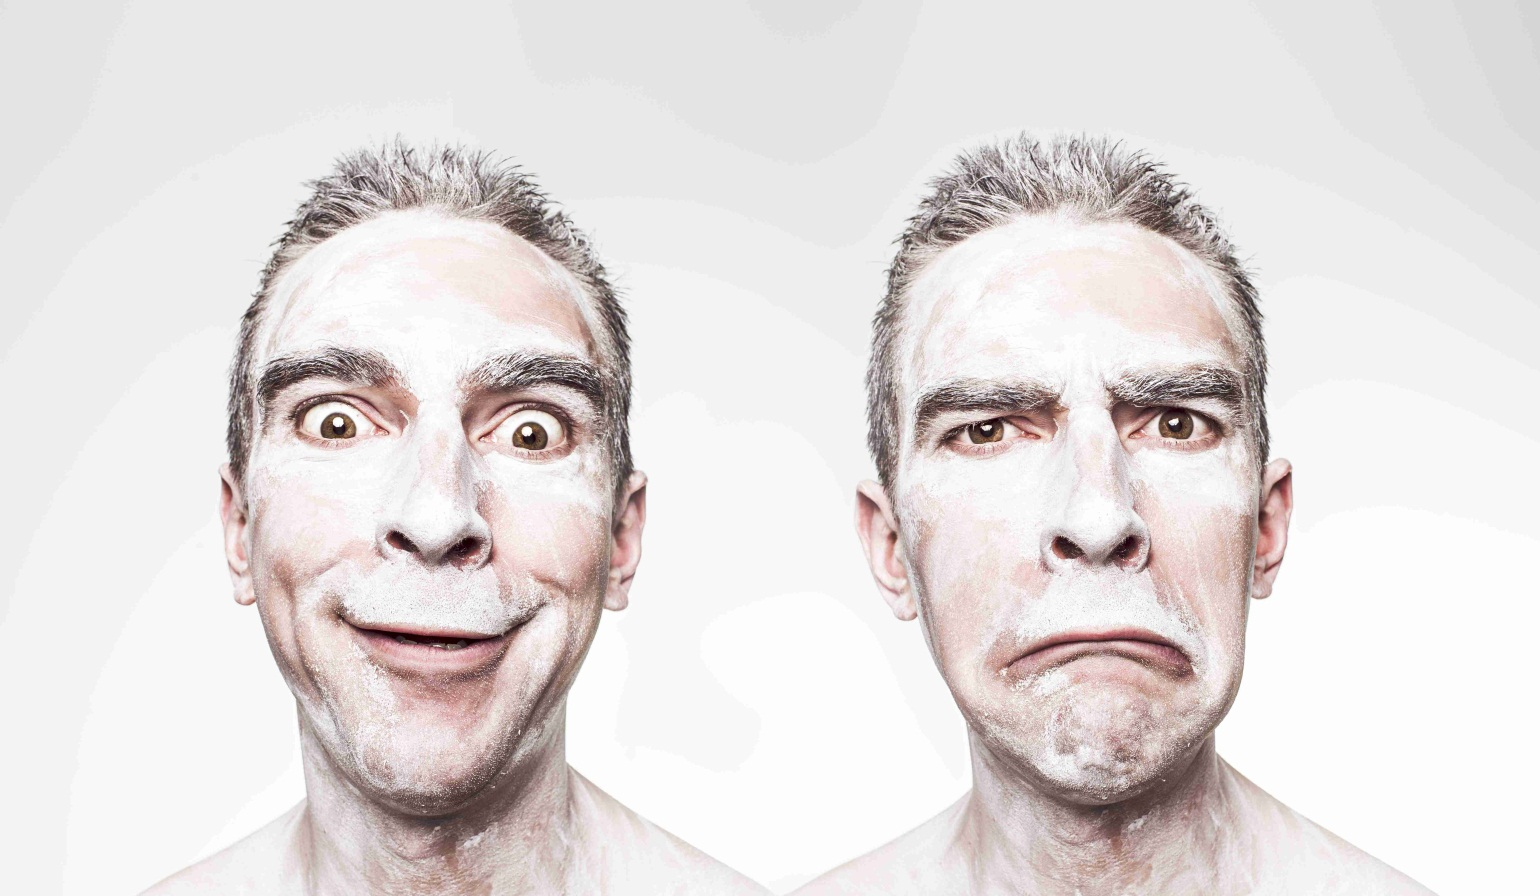
\includegraphics[width=8cm]{introduction_image.jpg}
  \end{figure}
  
\end{frame}

\begin{frame}
  \frametitle{Deliverables}

  \begin{itemize}
      \item Suitable results on classification of facial expressions
      \item Codebase
        \begin{itemize}
          \item Easy-to-use
          \item Well documented
          \item Extensible
      	\end{itemize}
  \end{itemize}
\end{frame}




\begin{frame}
  \frametitle{Mid-Level Discriminative Patch}

  \begin{itemize}
      \item  Part of an image describing a single feature
      \item Representative
      \item Different
      \item Detectable with high precision
  \end{itemize} 

  \vspace*{1.5cm}
  \small
  Singh et al., "Unsupervised discovery of mid-level discriminative patches.", Computer Vision-ECCV 2012: pp 73-86. (2012)

\end{frame}


\begin{frame}
  \frametitle{Example}
  \begin{figure}[t]
    \centering
    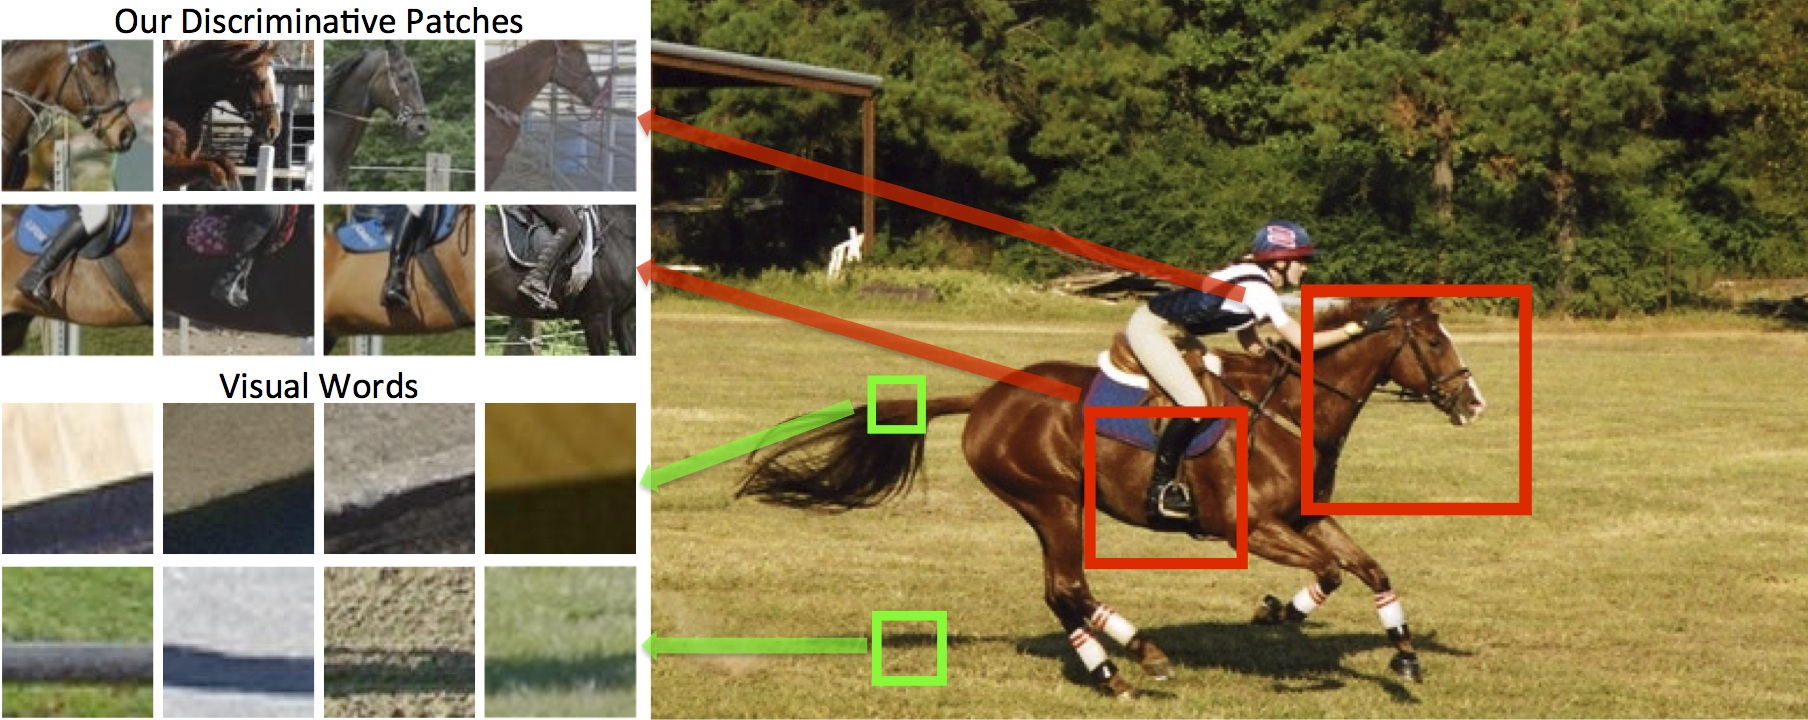
\includegraphics[width=11cm]{patches.jpg}
  \end{figure}
\end{frame}

\begin{frame}
  \frametitle{Discovery algorithm}
  \begin{figure}[t]
    \centering
    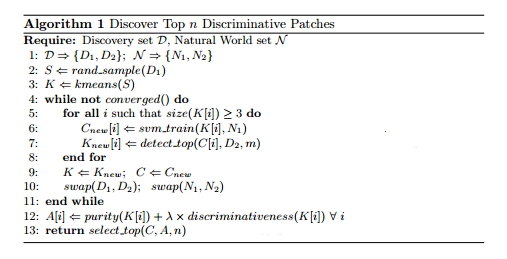
\includegraphics[width=10cm]{algorithm.png}
  \end{figure}
\end{frame}

\begin{frame}
  \frametitle{Code setup}
  
  CMake build configuration
  \begin{itemize}
      \item Platform independent
      \item Automatically generates C++ compiler and linker configurations
        \begin{itemize}
          \item Makefiles
          \item Visual Studio Project files
          \item ...
      	\end{itemize}
  \end{itemize}

\end{frame}

\begin{frame}
  \frametitle{Documentation setup}
  
  Doxygen
  \begin{itemize}
      \item Inline code documentation
      \item Extended comments
      \item Automatically generates HTML code interface documentation
  \end{itemize}

\end{frame}

\begin{frame}
  \frametitle{State of the application}
  \begin{itemize}
  	  \item Manual extraction of patches
      \item Setup of training and validation datasets
      \item Feature extraction using OpenCV HOGDescriptor
      \item Training and prediction through OpenCV SVM
  \end{itemize}
\end{frame}

\begin{frame}
  \frametitle{Manual Extraction}

  \begin{itemize}
      \item Dataset: 561(previous) + 700(added)
      \item Extracting the patches of mouth manually
        \begin{itemize}
          \item More accurate
          \item Perfect classifier
      	\end{itemize}
  \end{itemize}
\end{frame}

\begin{frame}
  \frametitle{Manual Extraction}
  \begin{figure}[t]
    \centering
    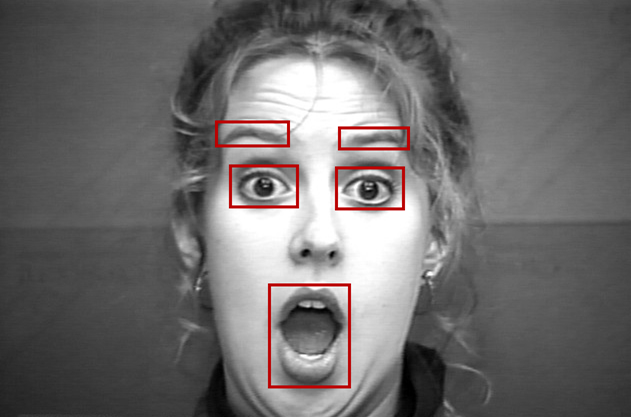
\includegraphics[width=8cm]{face.png}
  \end{figure}
\end{frame}

\begin{frame}
  \frametitle{Manual Extraction}

  \begin{itemize}
      \item Extracting the patches of mouth manually
        \begin{itemize}
          \item 96 * 96 pixels
          \item Be center of the patch\item Decrease uesless information
      	\end{itemize}
  \end{itemize}
  \begin{figure}[t]
    \centering
    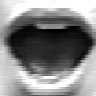
\includegraphics[width=2cm]{BW12_7.png}
    \centering
    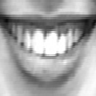
\includegraphics[width=2cm]{BW19_5.png}
      \centering
    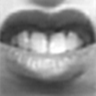
\includegraphics[width=2cm]{dis.png}
      \centering
    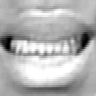
\includegraphics[width=2cm]{BW91_4.png}
  \end{figure}
\end{frame}

\begin{frame}
  \frametitle{Processing pipeline}
  \begin{itemize}
  	  \item Training and validation data
  	  \item Histogram equalization
      \item Feature extraction
      		\begin{itemize}
				\item  Histogram of oriented gradients
			\end{itemize}
      \item Train classifier on training data
        \begin{itemize}
			\item Support Vector Machine
		\end{itemize}
      \item Predict on validation data
  \end{itemize}
\end{frame}

% \begin{frame}
%   \frametitle{Histogram equalization}
% \begin{picture}(0,50) \put(0,-50){\hbox{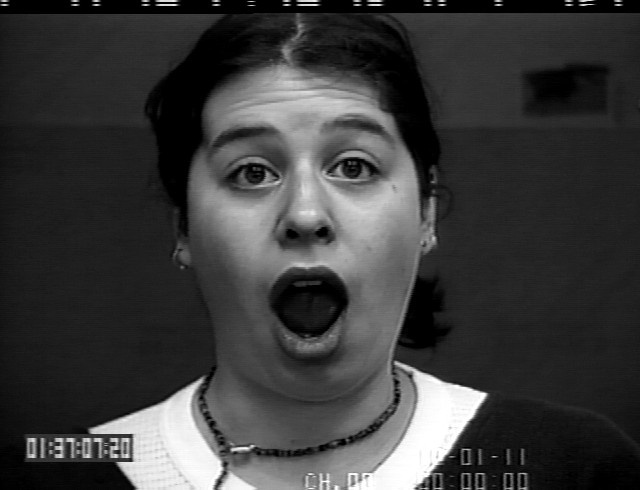
\includegraphics[scale=0.3]{images/BW78_7.png}}} 
% \end{picture} 
% \begin{picture}(0,50) \put(150,-50){\hbox{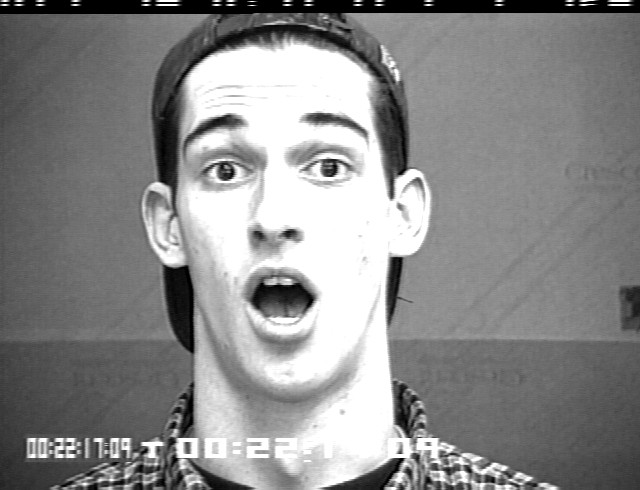
\includegraphics[scale=0.3]{images/BW56_7.png}}} 
% \end{picture} 
% \end{frame}

\begin{frame}[t]
  \frametitle{Histogram equalization}
  
  \begin{itemize}
 	\item Increase contrast
  \end{itemize}
  
\begin{picture}(0,50) \put(20,-100){\hbox{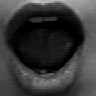
\includegraphics[scale=1.2]{images/BW78_7m.png}}} 
\end{picture} 
\begin{picture}(0,50) \put(180,-100){\hbox{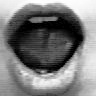
\includegraphics[scale=1.2]{images/p_33.jpg}}} 
\end{picture} 
\end{frame}

\begin{frame}
  \frametitle{Feature Extraction}
  \begin{columns}[onlytextwidth]
      \begin{column}{0.6\textwidth}
    \begin{itemize}
		\item 96x96 image size
        \item 8x8 cell size
        \item 9 histogram channels
        \item 4356 features per patch
	\end{itemize}
    
    \vspace{0.5cm}
     
        \begin{itemize}
			\item Sample size:
             \begin{itemize}
				\item 82 positive images
                \item 82 negative images
			\end{itemize}
		\end{itemize}
    
    \end{column}
    \begin{column}{0.4\textwidth}
      \centering
      %\rule{100pt}{150pt}% Place your graphic here
      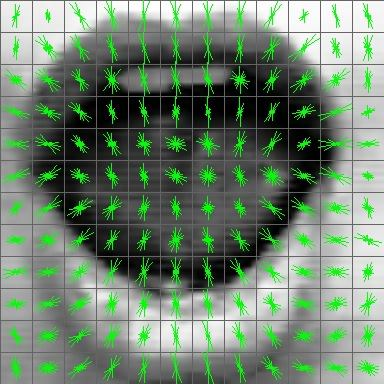
\includegraphics[scale=0.3]{slide3.jpg}
    \end{column}

​  \end{columns}
\end{frame}

\begin{frame}
  \frametitle{SVM Results}
        \begin{itemize}
			\item 96x96 pixel image size
		\end{itemize}
\begin{scriptsize}

  \begin{tabular}{| c | c | c | c | c | c |}
\hline


Channels & Features &  {Positive } & Negative  & Positive  & Negative \\

& & validation set & validation set & training set & training set \\
\hline

9 & 4356 & 100\% & 100\% & 100\% & 100\% \\

\hline

\end{tabular}

\end{scriptsize}




\end{frame}

\begin{frame}
  \frametitle{Overfitting}
    \begin{itemize}
		\item Number of features > number of samples
        \item Memorize data instead of generalize from learned trend
        \item Effect: Prediction on trained data better than on unknown data
	\end{itemize}
\end{frame}

\begin{frame}
  \frametitle{Adjust Relation of Samples to Features}
    \begin{itemize}
		\item Increase sample count
        	\begin{itemize}
				\item Flipping images vertically 
				\item 248 training patches, 40 validation patches
			\end{itemize}
    \vspace{0.5cm}
        \item Reduce feature dimensionality
        	\begin{itemize}
				\item Decrease pixels
				\item Decrease channels
				\item Apply Principal Component Analysis
			\end{itemize}
	\end{itemize}
\end{frame}

\begin{frame}
  \frametitle{Histogram of Oriented Gradients}
    \begin{itemize}
		\item Tuning parameters:
        	\begin{itemize}
				\item Patch size
				\item Histogram channels (Bins)
			\end{itemize}
	\end{itemize}
        \vspace{0.3cm}
          \centering
      %\rule{100pt}{150pt}% Place your graphic here
      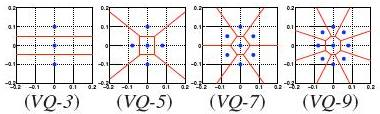
\includegraphics[scale=0.7]{bins.jpg}
\end{frame}

\begin{frame}
  \frametitle{Decrease Pixels}
    \begin{itemize}
		\item 32x32 Pixel image size

				\item 8x8 pixels cell size

				\item 9 Bins
	\end{itemize}
    \vspace{1.0cm}
 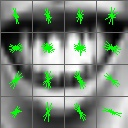
\includegraphics[width=3cm,height=3cm]{images/negativeTrain_14_32.jpg}
    \hspace{0.7cm}
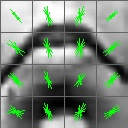
\includegraphics[width=3cm,height=3cm]{images/negativeTrain_63_32.jpg}
    \hspace{0.7cm}
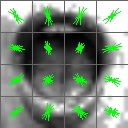
\includegraphics[width=3cm,height=3cm]{images/positiveTrain_25_32.jpg}
   

\end{frame}

\begin{frame}
  \frametitle{Patch size 32x32}
  
\begin{scriptsize}
 
\begin{tabular}{| c | c | c | c | c | c |}
\hline
Bins & Features &  Positive  & Negative  & Positive  & Negative \\

& & validation set & validation set & training set & training set \\

\hline
9 & 324 & 90\% & 100\% & 100\% & 96\% \\
7& 252 & 90\% & 100\% & 100\% & 96\% \\
5& 180 & 90\% & 100\% & 100\% & 95\% \\
\hline
\end{tabular}

\end{scriptsize}

\end{frame}
\begin{frame}
  \frametitle{Decrease Pixels}
    \begin{itemize}
		\item 16x16 Pixel image size

				\item 8x8 pixels cell size

				\item 9 Bins
	\end{itemize}
    \vspace{1.0cm}
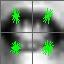
\includegraphics[width=3cm,height=3cm]{hog16.jpg}
    \hspace{0.7cm}
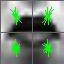
\includegraphics[width=3cm,height=3cm]{hog16b.jpg}
    \hspace{0.7cm}
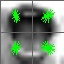
\includegraphics[width=3cm,height=3cm]{images/positiveTrain_25_16.jpg}

\end{frame}



\begin{frame}
  \frametitle{Patch size 16x16}
  
\begin{scriptsize}  
\begin{tabular}{| c | c | c | c | c | c |}
\hline
Bins & Features &  Positive  & Negative  & Positive  & Negative \\

& & validation set & validation set & training set & training set \\
\hline
9 & 36 & 92\% & 55\% & 91\% & 47\% \\
7& 28 & 100\% & 47\% & 95\% & 43\% \\
5& 20 & 100\% & 30\% & 99\% & 34\% \\
\hline
\end{tabular}
\end{scriptsize}
\end{frame}

\begin{frame}
  \frametitle{Principal Component Analysis}
  \begin{scriptsize} 
\begin{tabular}{| c | c | c | c | c | c |}
\hline
Bins & Features &  Positive  & Negative  & Positive  & Negative \\

& & validation set & validation set & training set & training set \\
\hline
9 & 81 & 55\% & 35\% & 74\% & 50\% \\
7& 49 & 47\% & 15\% & 61\% & 29\% \\
5& 25 & 75\% & 2\% & 59\% & 19\% \\
\hline
\end{tabular}
\end{scriptsize} 
\end{frame}


\begin{frame}

  \frametitle{Generating additional images}
  
  \begin{itemize}
      \item A Gaussian blur filter was used to generate variations of each image
      \item 32 variations of each image were created with different blur levels
  \end{itemize}
  
\end{frame}

\begin{frame}
  \frametitle{Adding blurred images}
\begin{tabular}{| c | c | c |}
\hline
Expression & Positive  & Negative \\
& validation set & validation set \\
\hline
Happy & $100 \%$ & 98\% \\
Anger & $100\%$ & 97\% \\
Surprise & $100\%$ & $100\%$  \\
\hline
\end{tabular}
\end{frame}

\begin{frame}
  \frametitle{Future steps}
  \begin{itemize}
  	  \item Unsupervised cluster detection (K-means).
      \item Inclusion of patches apart from mouth.
      \item Comparing the results k-means with manual extraction. 
      \item Dimensionality reduction (if need be) using techinques such as PCA, LDA, etc.
 
  \end{itemize}

\end{frame}

\begin{frame}
  \frametitle{References}
  \begin{itemize}
  	  \item Singh et al., "Unsupervised discovery of mid-level discriminative patches", Computer Vision-ECCV 2012: pp 73-86. (2012)
      \item Doersch et al. "What makes Paris look like Paris?." , ACM Transactions on Graphics 31, no. 4 (2012)

  \end{itemize}

\end{frame}



\begin{frame}
  \frametitle{Questions?}
  
  \begin{center}
  \LARGE Thank you for your attention
  \end{center}
\end{frame}

% Example slides from here on, will be removed

% Image placement
\begin{frame}
  \frametitle{Image placement example}
\begin{picture}(0,50) \put(70,-50){\hbox{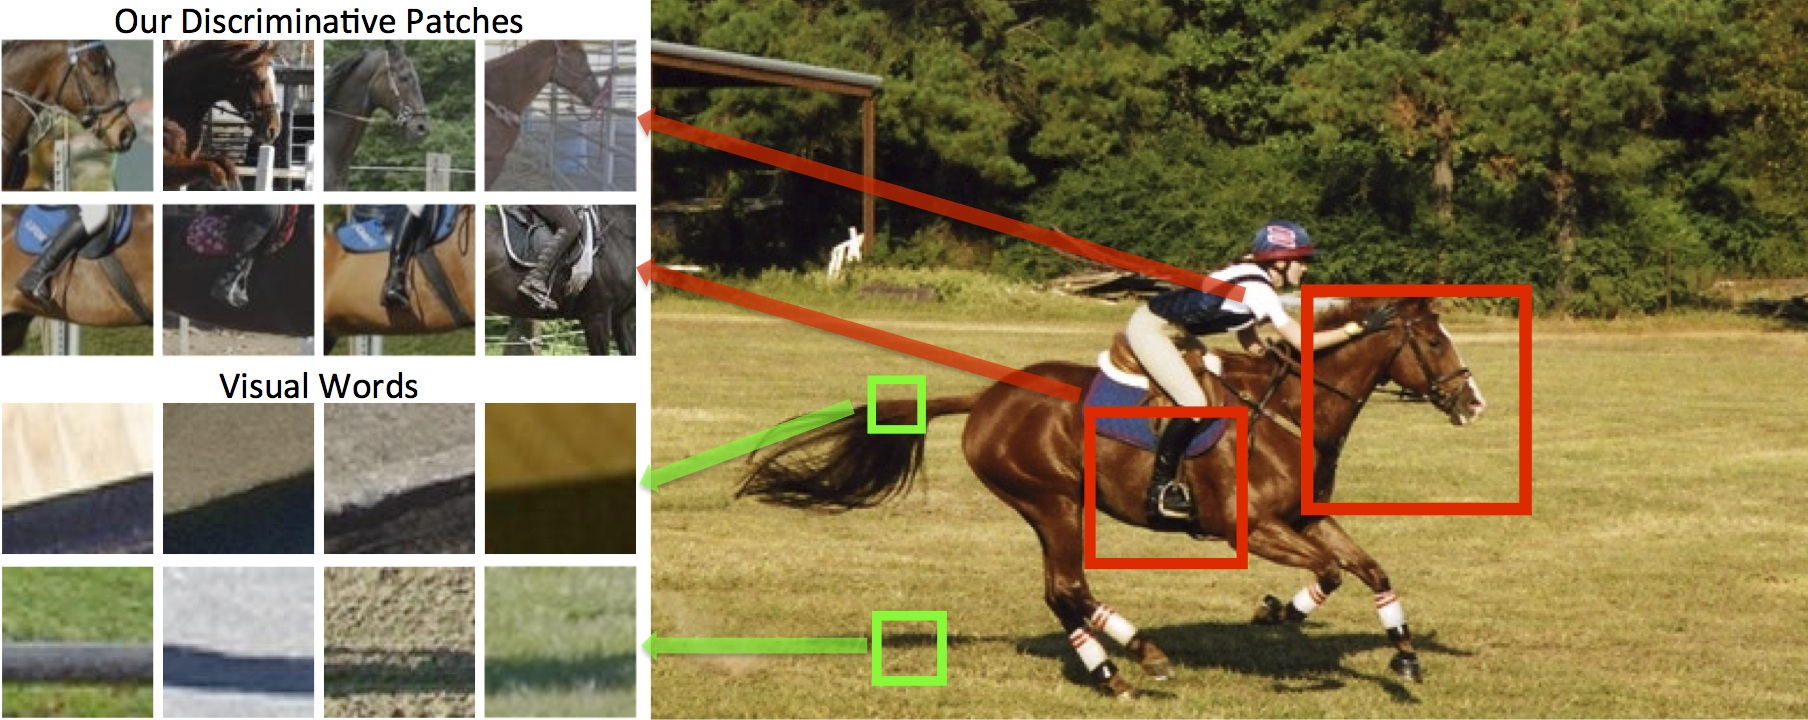
\includegraphics[scale=0.1]{patches.jpg}}} 
\end{picture} 
\begin{picture}(0,50) \put(200,-50){\hbox{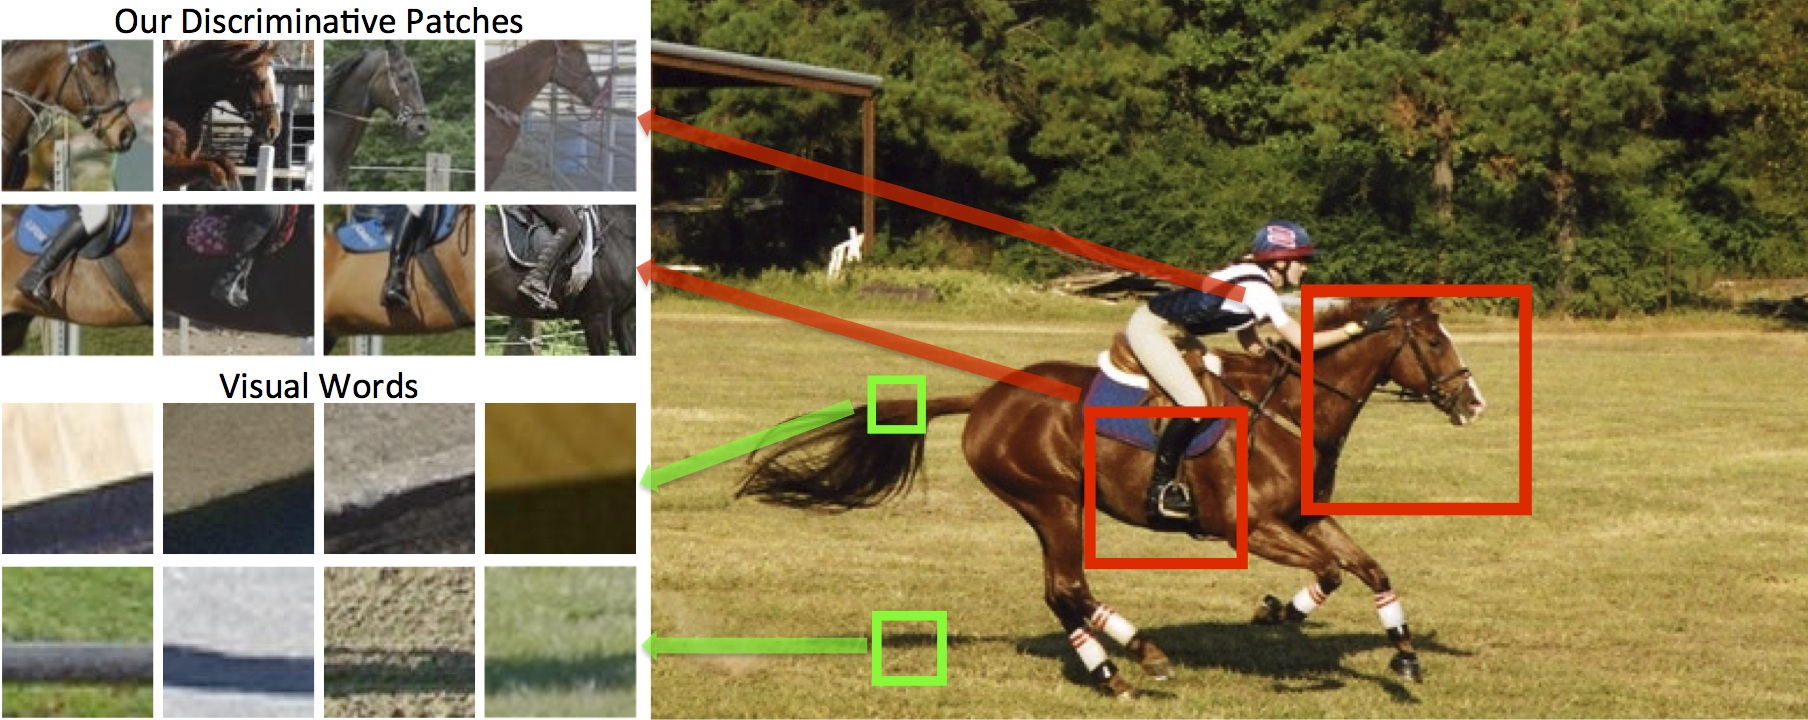
\includegraphics[scale=0.1]{patches.jpg}}} 
\end{picture} 
\end{frame}

\begin{frame}
  \frametitle{2 columns}
  \begin{columns}[onlytextwidth]
    \begin{column}{0.6\textwidth}
      \centering
      %\rule{100pt}{150pt}% Place your graphic here
      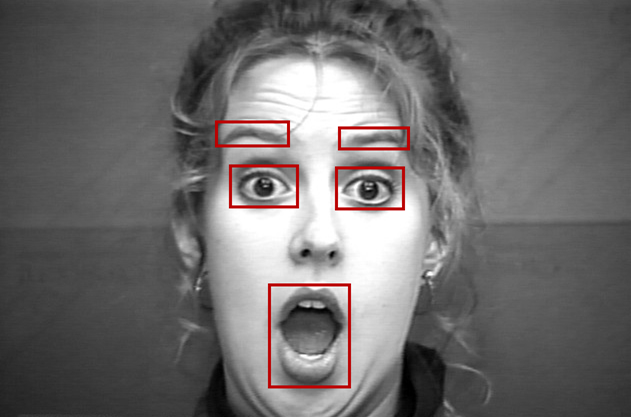
\includegraphics[scale=0.4]{face.png}
    \end{column}
    \begin{column}{0.4\textwidth}
    Here is some regular text in a column.
    \newline
    Here is some more text.
    \end{column}
​  \end{columns}
\end{frame}

\begin{frame}
  \frametitle{2x2 images}

\begin{columns}[t]
\column{.5\textwidth}
\centering
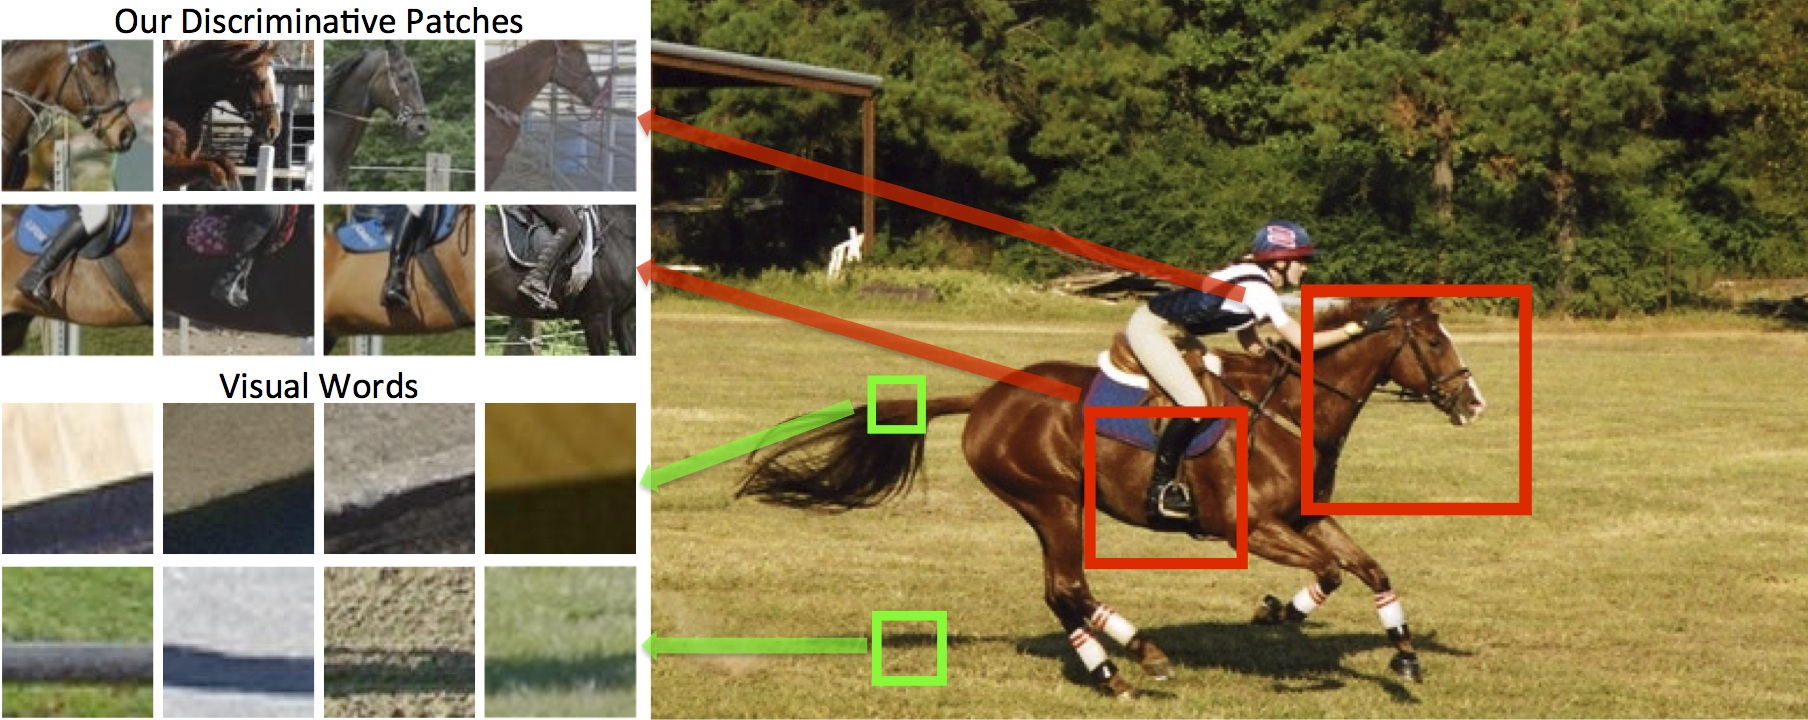
\includegraphics[width=5cm,height=4cm]{patches.jpg}\\
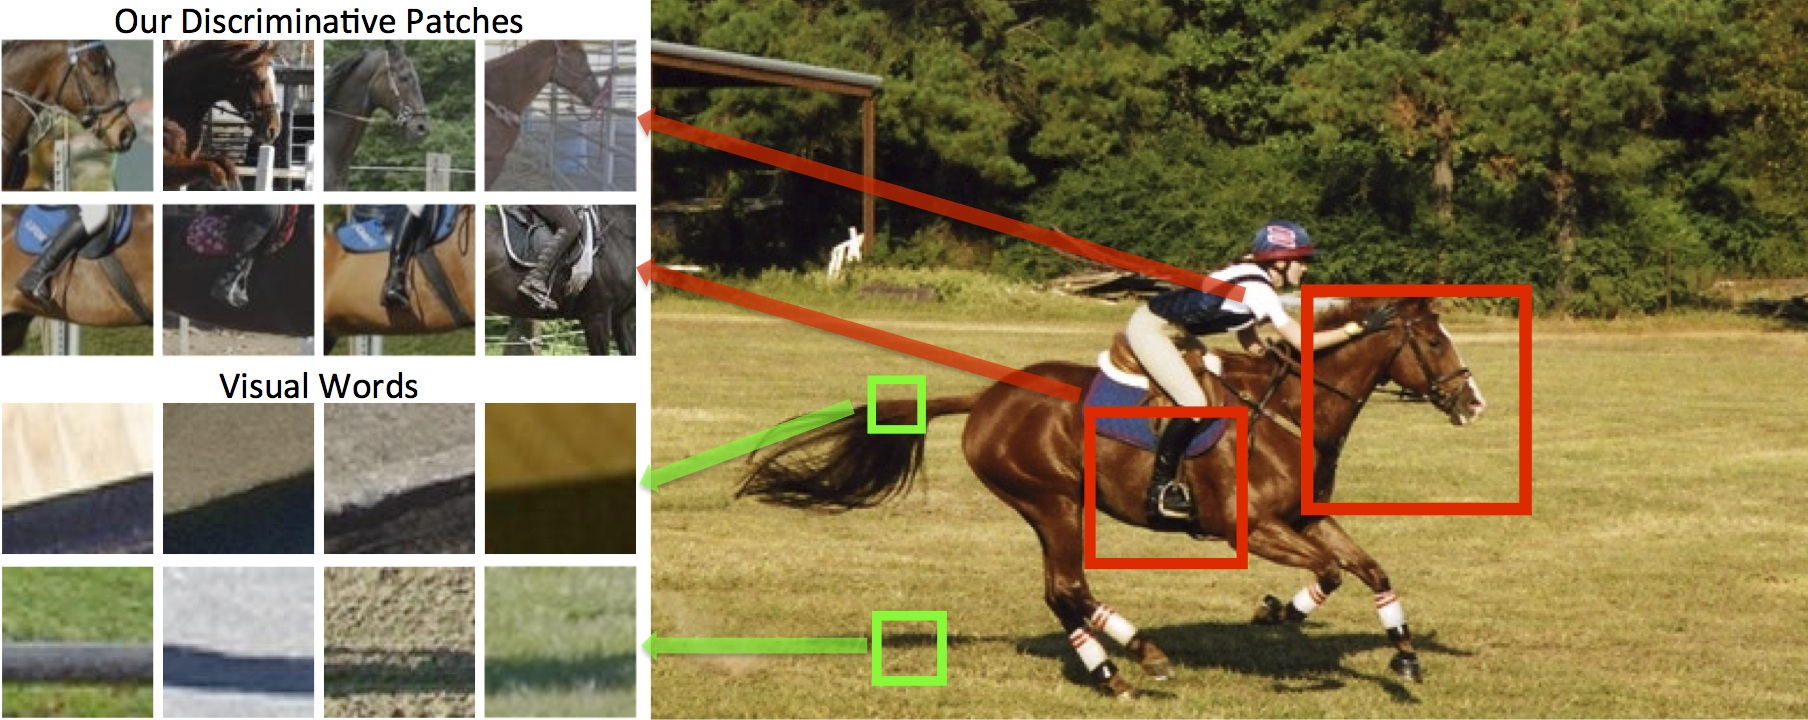
\includegraphics[width=5cm,height=4cm]{patches.jpg}
\column{.5\textwidth}
\centering
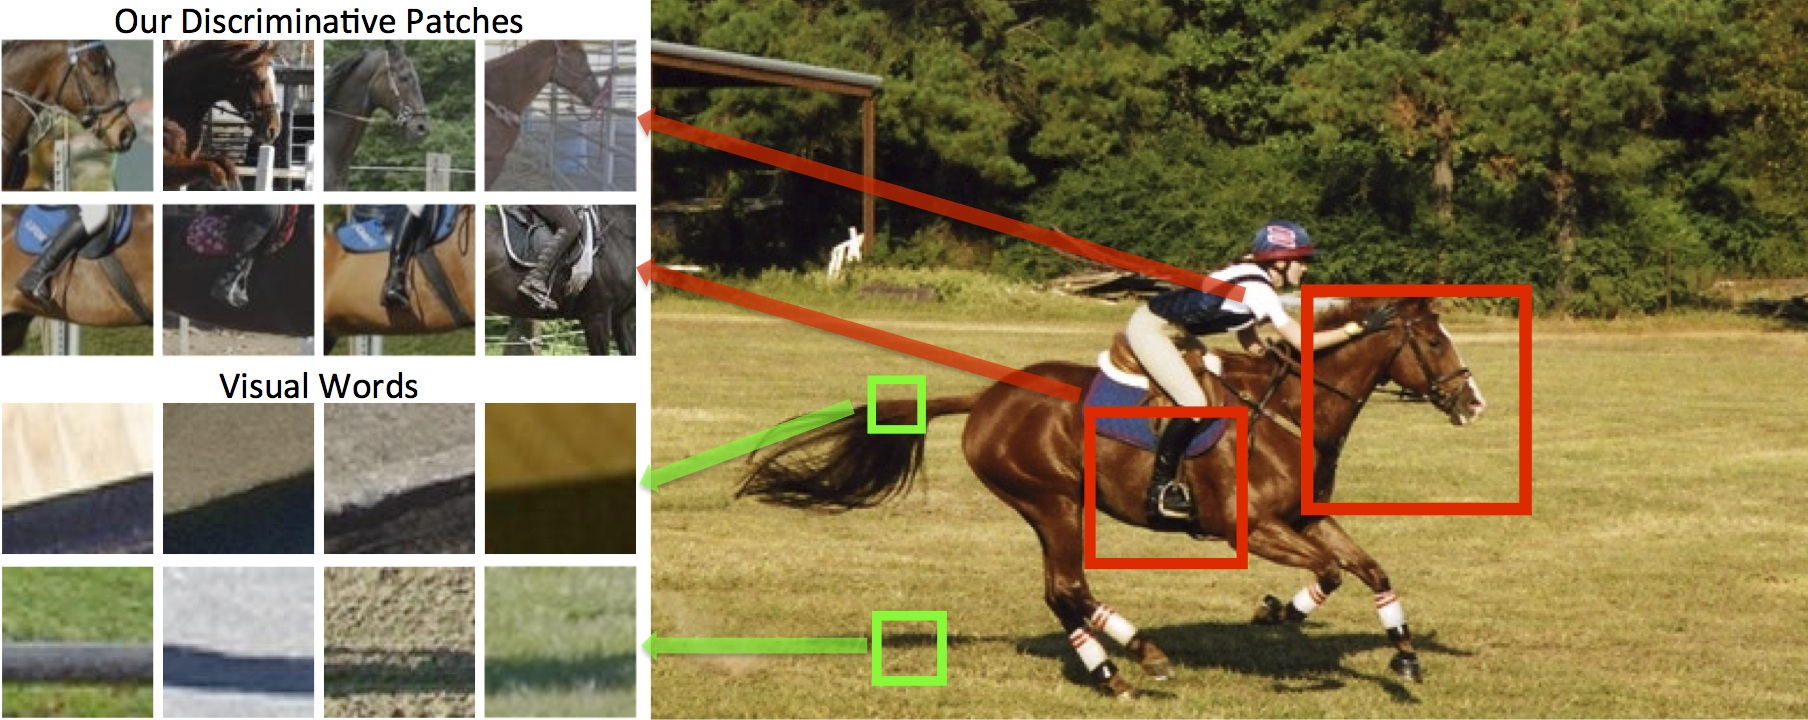
\includegraphics[width=5cm,height=4cm]{patches.jpg}\\
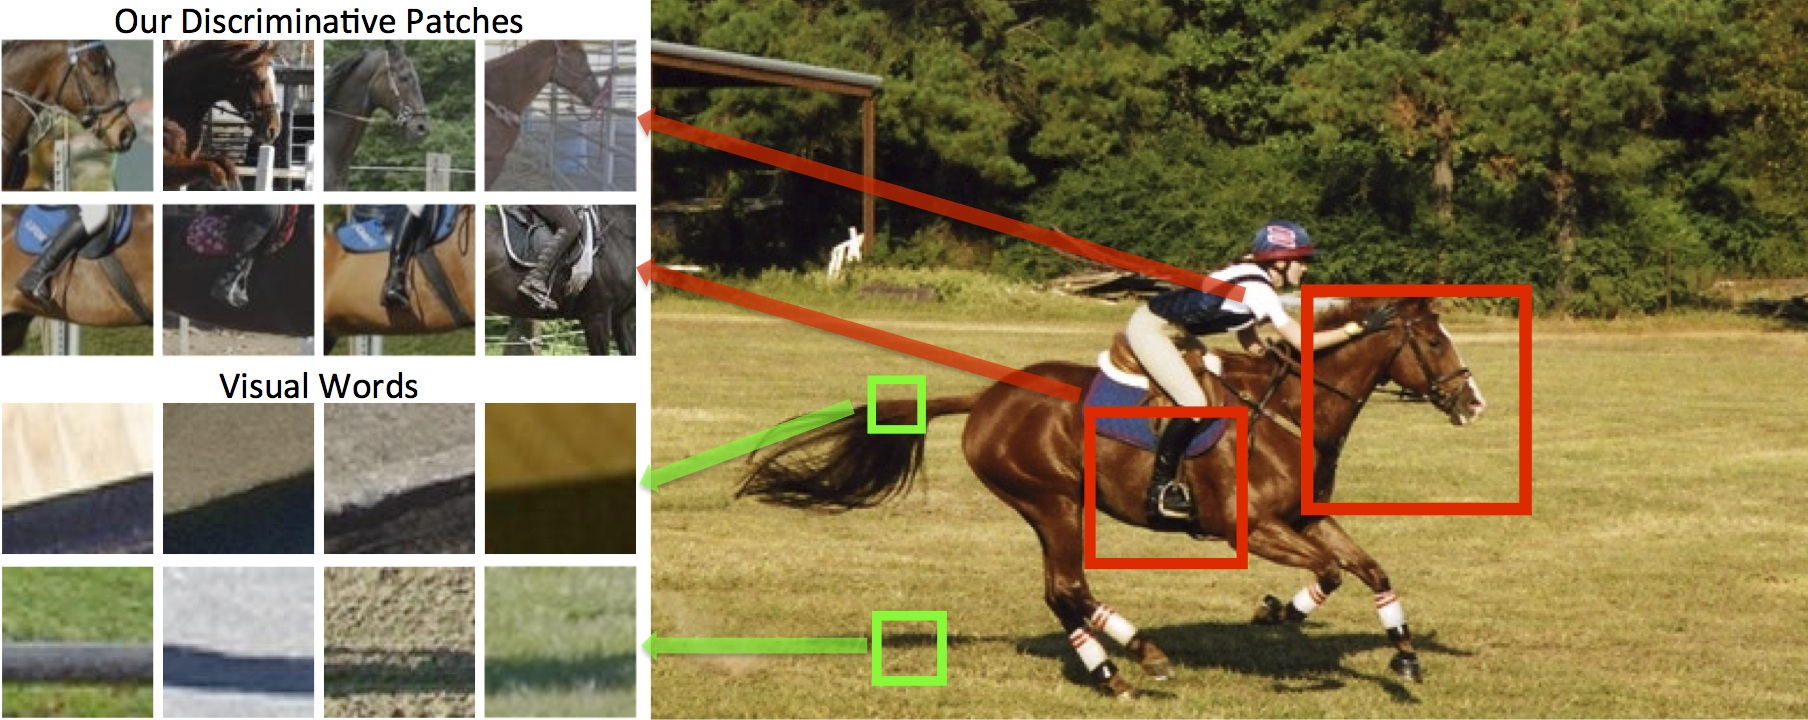
\includegraphics[width=5cm,height=4cm]{patches.jpg}
\end{columns}
\end{frame}

\begin{frame}
  \frametitle{Bullet points example}
  % With \pause bullet points appear 1 by 1, otherwise all at once
  Things in a Bulleted List\pause
  \begin{itemize}
  \item Bullets that\pause
  \item Come up\pause
  \item One by one %leave out the \pause on the final item
  \end{itemize}
\end{frame}




\end{document}
